\chapter{Symbol and characteristic variety}\label{chapter:characteristics}%
\chapterSummary{We define the notion of symbol of a system of partial differential equations.}
\section{The problem}
The Cauchy--Kovalevskaya theorem\SubIndex{Cauchy--Kovalevskaya theorem}\SubIndex{theorem!Cauchy--Kovalevskaya} says that we can solve a system of differential equations, if we can write it as solving for the highest derivative in a single variable \(t\) in terms of all other derivatives.
If we can't do this in the variables we are given, we might be able to do it after a change of variables. 
So we need a coordinate free description of ``how many derivatives'' are taken in a given direction.
\begin{example}The Laplace operator in the plane: \(u \mapsto u_{xx}+u_{yy}\).
At first glance, it appears to take two derivatives along each coordinate axis, and no derivatives in any other directions.
But the Laplace operator is invariant under rotation, so it actually ``feels'' the second derivatives in all directions.
\end{example}

\section{The symbol of a linear operator}
If you differentiate a high frequency wave in a direction in which it oscillates, it gets bigger.
If you differentiate in a direction in which the wave is constant, it gets killed.
We detect derivatives by plugging in waves.

Take a large number \(\lambda\) and any function \(f(x)\) vanishing at the origin.
Near the origin, the function \(e^{i\lambda f}\) looks like a high frequency wave: expand \(f\) in a Taylor series \(f(x)=\sum \xi_i x_i + \dots\),
\[
e^{i\lambda f} = e^{i \lambda \sum \xi_i x_i + \dots}.
\]
\begin{center}
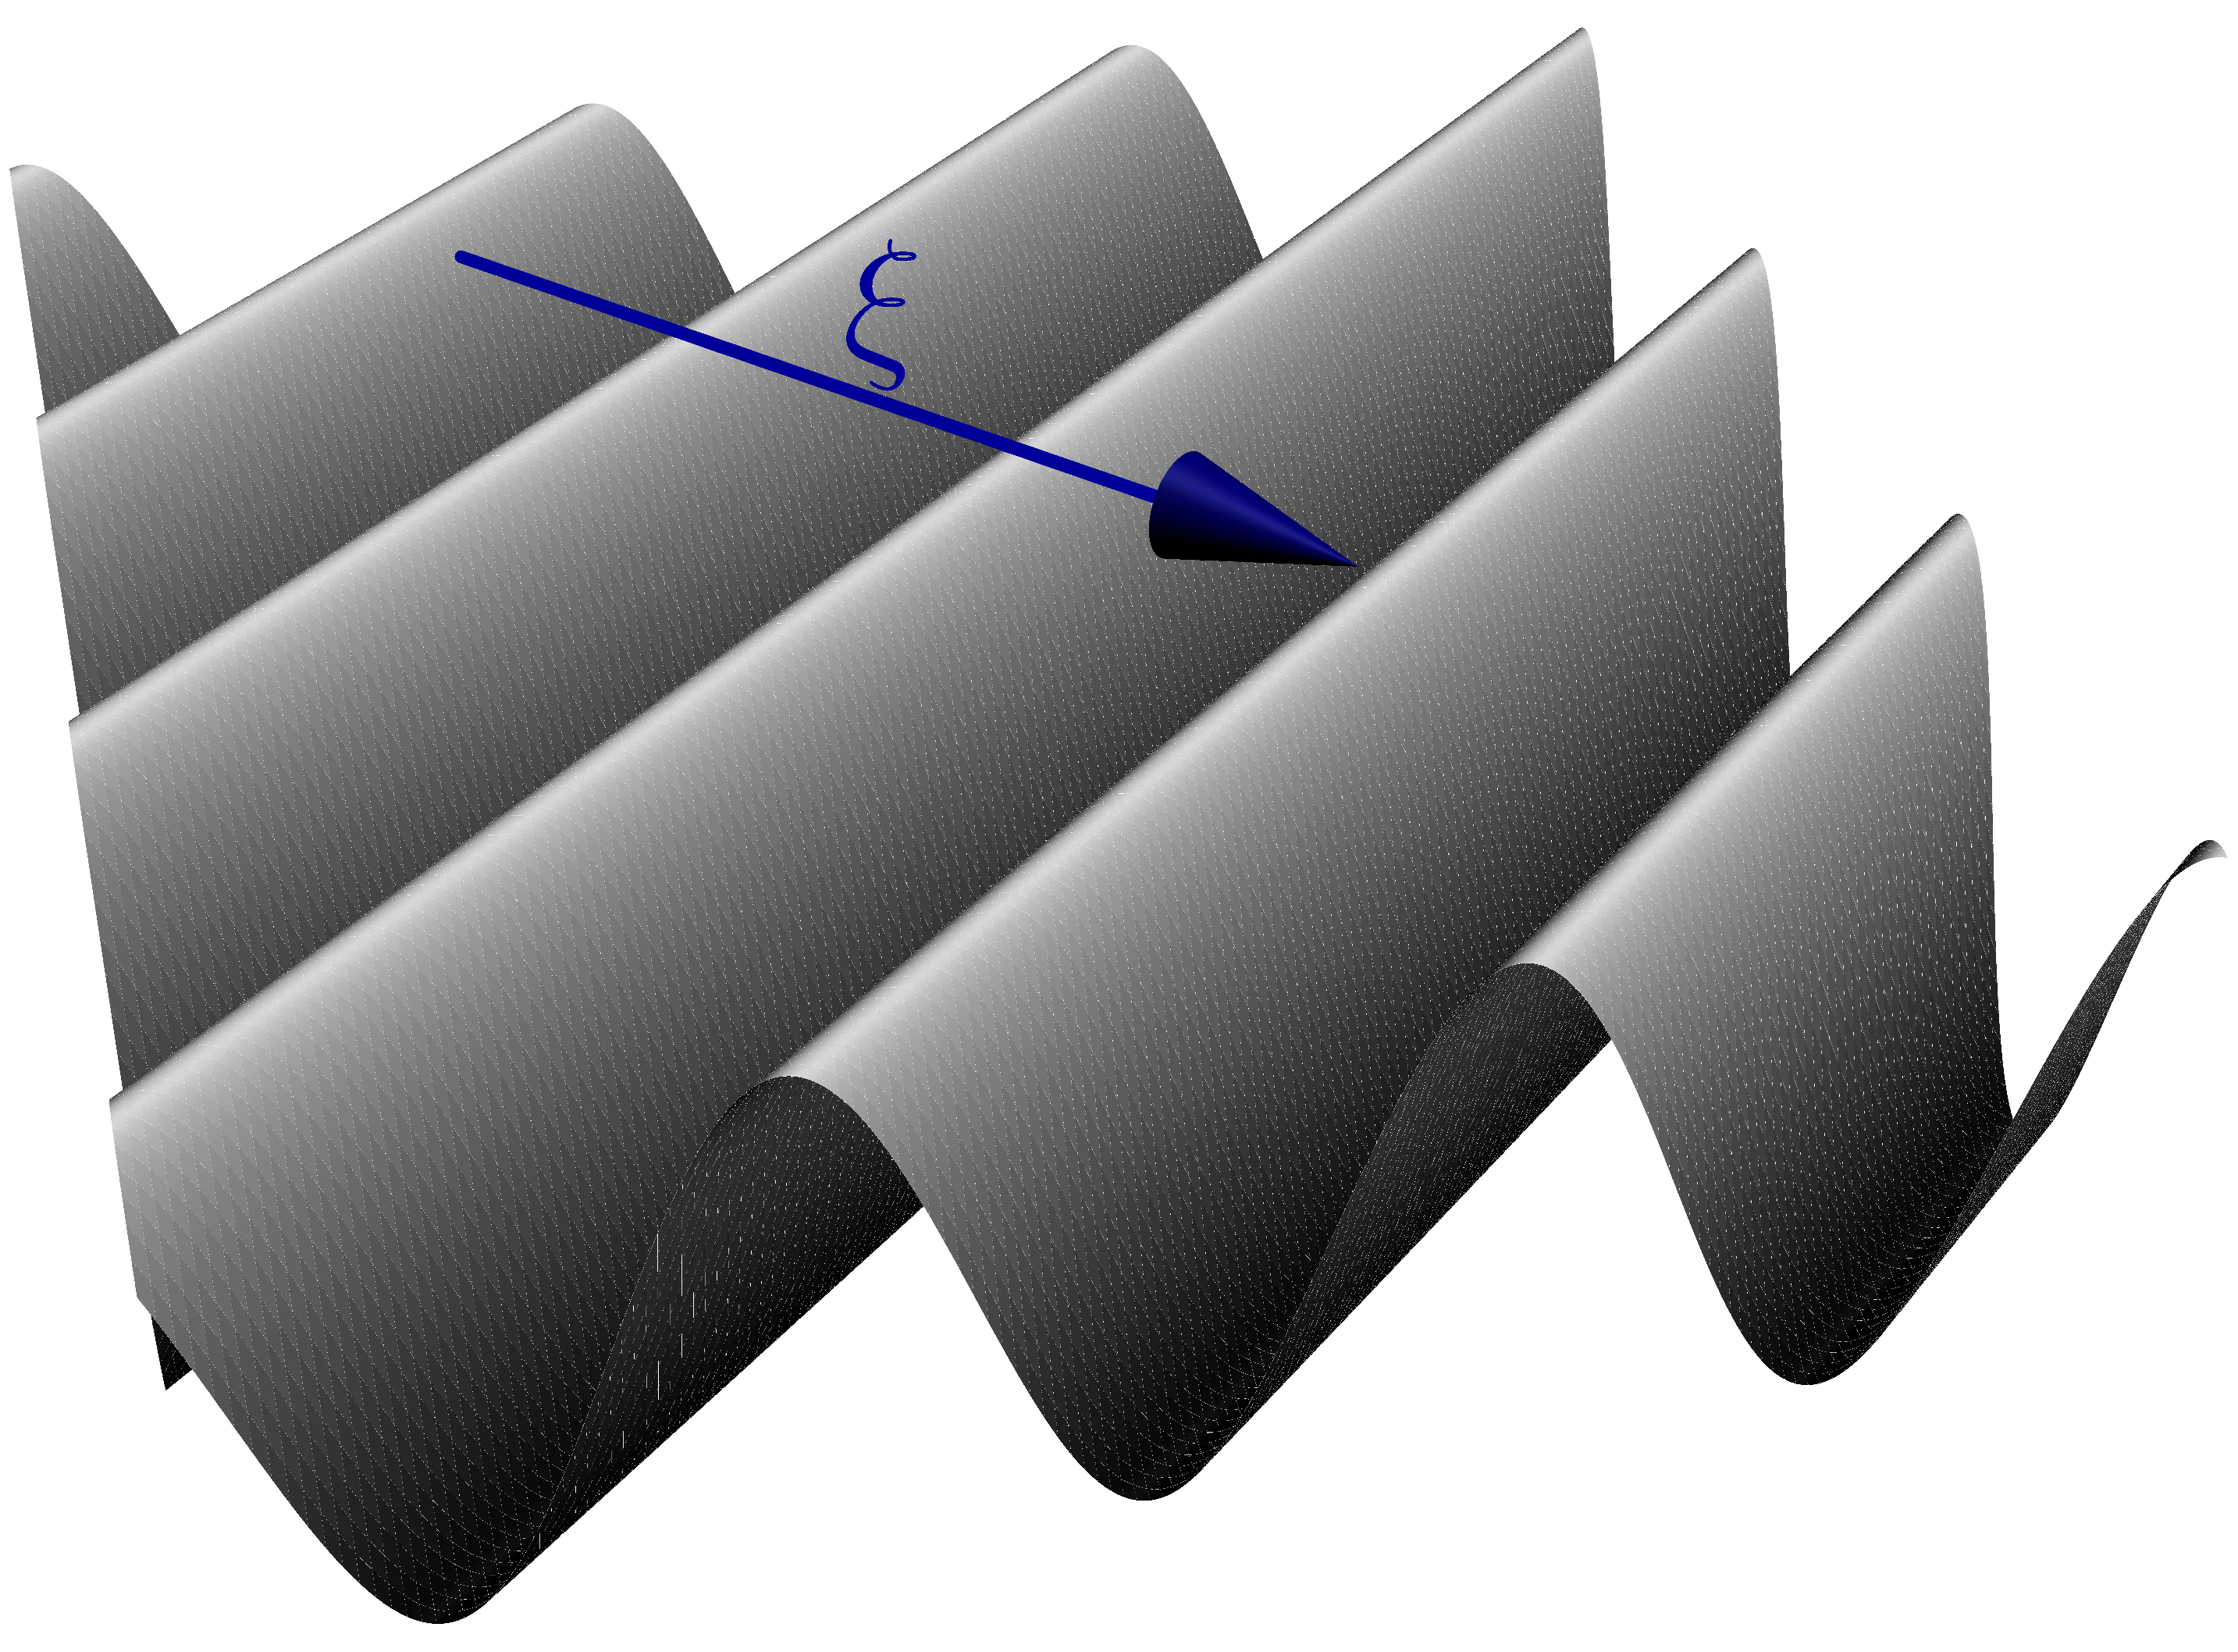
\includegraphics[width=4cm]{wave}
\end{center}
Any linear differential operator,
\[
P=\sum_{|a|\le m} c_a(x) \partial^a
\]
is a polynomial \(P=P(x,\partial)\) in the operators \(\p{x_i}\); the coefficients are functions of \(x\).
Write this polynomial
\[
P(x,\xi)=
\sum_{|a|\le m} c_a(x) \xi^a.
\]
Let \(P_m\) be the highest order terms, also called the \emph{symbol}:\define{symbol}
\[
P_m(x,\xi)=\sum_{|a|=m} c_a(x) \xi^a,
\]
also denoted \(\opsymbol[P]{\xi}\), for \(\xi=\xi_i dx^i \in T^* M\) a \(1\)-form.
To see ``how many derivatives'' \(P\) takes in some direction, expand:
\[
e^{-i\lambda f}P\left[e^{i \lambda f}u\right]
=
\sum_{|a|\le m} e^{-i\lambda f}c_a(x) \partial^a \pr{e^{i\lambda f}u},
\]
Every time a derivative hits \(e^{i\lambda f}u\), it either hits the exponential factor, pulling down a power of \(\lambda\), or hits the \(u\), so no power of \(\lambda\).
So the leading order term in \(\lambda\) is
\begin{align*}
e^{-i\lambda f}P\left[e^{i \lambda f}u\right]
&=i^m \lambda^m \sum_{|a|=m} c_a(x) \xi^a u + O(\lambda)^{m-1},
\\
&=i^m\lambda^mP_m(x,\xi)u+O(\lambda)^{m-1}.
\end{align*}
where \(\xi=df(x)\).
Without taking coordinates,
\[
\opsymbol[P]{df}u=\lim_{\lambda \to \infty} \frac{e^{-i\lambda f} P \left[e^{i\lambda f}u\right]}{i^m\lambda^m}
\]
for any continuously differentiable function \(f\) vanishing at \(x\).
\begin{example}
The heat operator in the plane is
\[
Pu=u_t-u_{xx}-u_{yy}
\]
for a function \(u=u(t,x,y)\), and the symbol is \(\opsymbol[P]{c \, dt + a \, dx + b \, dy}=-a^2-b^2\).
\end{example}

All along we could have allowed \(u\) to be valued in, say, \(\R[q]\), and allow the coefficients \(c_a(x)\) to be \(p \times q\) matrices.
Then \(\opsymbol[P]{\xi}\) is a \(p \times q\) matrix.
The matrix entries are functions of \(x\) and polynomials of degree \(m\) in \(\xi\).
\prob{characteristic.variety:CR}{Find the symbol of the Cauchy--Riemann operator
\[
P\begin{bmatrix}u \\v\end{bmatrix}=
\begin{pmatrix}
u_x-v_y\\
u_y+v_x
\end{pmatrix}.
\]}
\begin{answer}{characteristic.variety:CR}
\[
P(x,y,\p{x},\p{y})
=
\begin{pmatrix}
\p{x}&-\p{y}\\
\p{y}&\p{x}
\end{pmatrix}
\]
so turning derivatives \(\p{x},\p{y}\) into Greek variables \(\xi,\eta\):
\[
P(x,y,\xi,\eta)
=
\begin{pmatrix}
\xi&-\eta\\
\eta&\xi
\end{pmatrix}.
\]
\end{answer}
\begin{problem}{characteristic.variety:rescale}
If we are interested in a linear system of \emph{equations} \(0=Pu\), rather than an operator \(P\), the equations have the same solutions if we rescale both sides by some invertible matrix \(g(x)\).
Similarly, we could rescale the \(u\) variable by a matrix \(h(x)\).
Check that 
\[
\opsymbol[gPh]{\xi}=g\opsymbol[P]{\xi}h.
\]
\end{problem}
If we change variables by a diffeomorphism \(y=h(x)\), then \(\partial_{x_i} = \sum_j \pderiv{y_j}{x_i} \partial_{y_j}\) and for any \(1\)-form \(\xi=\sum_j \xi_j dy_j=\sum_{ij} \xi_j \pderiv{y_j}{x_i} dx_i\), so when we substitute \(\xi_i\) for \(\partial_{y_i}\), 
\[
\opsymbol[h_* P]{\xi} = \opsymbol[P]{h^*\xi}.
\]
We knew this already: the symbol \(\opsymbol[P]{\xi}\) is defined independently of coordinates.
\begin{example}
Taking exterior derivative \(d\) as our differential operator,
\[
e^{-i \lambda f} d(e^{i \lambda f}) = i\lambda df \wedge \omega + d\omega,
\]
so the symbol is
\[
\opsymbol[d]{\xi}=\xi \wedge,
\]
i.e. the symbol is the linear transformation \(\omega \mapsto \xi \wedge \omega\), where \(\xi\) is a \(1\)-form.
\end{example}

\section{Background material from projective geometry}
The \emph{projective space}\define{projective space} \(\Proj(V)\) of a vector space \(V\), over any field, is the set of lines through the origin of \(V\) \cite{Onishchik/Sulanke:2006}. If \(V\) has dimension \(n+1\), we may write \(\Proj(V)\) as \(\Proj^n\).
For any \(v \in V\) with \(v \ne 0\), \([v] \in \Proj(V)\) is the line through \(v\).
Any nonzero linear function \(f\) on \(V\) vanishes on a hyperplane in \(V\).
This hyperplane determines \(f\) up to rescaling, and vice versa.
So each point \([f]\) of \(\Proj(V^*)\) is naturally identified with a hyperplane in \(V\).

\section{The characteristic variety}
The \emph{characteristic variety}\define{characteristic!variety} of a linear differential operator \(P\) is
\[
\charvariety[P]{m} = \Set{[\xi] \in \Proj(T^*_m M)|\ker \opsymbol[P]{\xi} \ne 0}.
\]
Let \(T_m^{\C*}M\defeq T_m^*M \otimes \C\).
The \emph{complex characteristic variety} consists of complex lines in a complex vector space:
\[
\complexcharvariety[P]{m} = \Set{[\xi] \in \Proj(T^{\C*}_m M) | \ker \opsymbol[P]{\xi} \ne 0}.
\]
A \(1\)-form \(\xi\) belongs to the characteristic variety just when the operator \(P\) takes ``exceptionally few'' derivatives in the direction of \(\xi\).
\begin{example}
For the heat operator, the characteristic variety is the set of \([c,a,b] \in \Proj^2\) so that \(a^2+b^2=0\), i.e. the single point \([c,a,b]=[1,0,0] \in \Proj^2\), while complex characteristic variety consists of the complex number solutions to the same equations: \([c,a,\pm a]\), i.e. \(b=ia\) and \(b=-ia\), a union of two complex lines.
\end{example}
\begin{example}
Take exterior derivative \(d\) on \(k\)-forms as our differential operator.
The symbol is
\(\opsymbol[d]{\xi}= \xi \wedge\), so the characteristic variety is the set of all lines \([\xi]\) spanned by \(1\)-forms \(\xi \ne 0\) so that \(\xi \wedge \omega=0\) for some \(\omega \ne 0\). 
If we work with only \(0\)-forms \(\omega\), then this forces \(\xi=0\): the characteristic variety is empty.
If \(k>0\), then any \(\xi\) has \(\xi \wedge \omega=0\) for some \(\omega \ne 0\): take any \(\omega\) of the form \(\xi \wedge \eta\).
So the characteristic variety of the exterior derivative on \(k\)-forms is
\[
\charvariety[d]{m} = 
\begin{cases}
\varnothing, & \text{ if \(k=0\)}, \\
\Proj(T^*_m M), & \text{ if \(k>0\)}.
\end{cases}
\]
The same calculation computes the complex characteristic variety:
\[
\complexcharvariety[d]{m} = 
\begin{cases}
\varnothing, & \text{ if \(k=0\)}, \\
\Proj(T^{\C*}_m M), & \text{ if \(k>0\)}.
\end{cases}
\]
\end{example}
\begin{example}
For the heat operator, the characteristic variety at each point consists of the single hyperplane \(dt=0\).
This hyperplane is the tangent plane to each surface representing space at constant time.
\end{example}
\begin{example}
For a vector field \(X\), thought of as a differential operator \(Pu=Xu\), the characteristic variety is the set of \([\xi]\) so that \(\xi(X)=0\), i.e. the set of all hyperplanes containing the vector \(X\).
\end{example}
\begin{example}
For the wave operator, \(Pu=u_{tt}-u_{xx}-u_{yy}\), the symbol is \(\opsymbol[P]{t,x,y,c,a,b}=c^2-a^2-b^2\).
Up to rescaling, we can arrange \(c=1\), so the characteristic variety is a circle \([1,a,b] \in \Proj^2\) so that \(a^2+b^2=1\).
As a family of hyperplanes, this circle is the set of hyperplanes tangent to the ``light cone'' \(dt^2=dx^2+dy^2\).
\end{example}
Points of the complex characteristic variety are complex hyperplanes in the spaces of complexified tangent vectors.
\prob{char.var:Maxwell}{Find the characteristic variety of Maxwell's equations in the vacuum.}
\begin{answer}{char.var:Maxwell}
If we write each antisymmetric matrix
\[
\begin{pmatrix}
0 & z & -y \\
-z & 0 & x \\
y & -x & 0
\end{pmatrix}
\]
as \([x,y,z]\), Maxwell's equations become
\begin{align*}
\p{t}E&=[\p{x},\p{y},\p{z}]H,\\
\p{t}H&=-[\p{x},\p{y},\p{z}]E.
\end{align*}
As an operator
\[
P\begin{bmatrix}E\\H\end{bmatrix}
=
\begin{pmatrix}
\p{t}I & -[\p{x},\p{y},\p{z}]\\
[\p{x},\p{y},\p{z}] & \p{t}I
\end{pmatrix}
\]
so if we write \(1\)-forms as \(\xi\,dx+\eta\,dy+\zeta\,dz+\tau\,dt\),
the symbol matrix is
\[
\opsymbol{P}
=
\begin{pmatrix}
\tau I & -[\xi,\eta,\zeta]\\
[\xi,\eta,\zeta] & \tau I
\end{pmatrix}
\]
a square matrix with determinant
\[
\left(\tau^2 - \xi^2 - \eta^2 - \zeta^2\right)^2 \tau^2.
\]
The characteristic variety consists of the hyperplanes tangent to the light cone and the hyperplane \(\tau=0\) tangent to space at constant time.
\end{answer}

\section{Linearization}
\begin{example}
Take a nonlinear differential equation, say \(u_t=u_{xx} u + \sin\of{u_x}\), and take a solution \(u(t,x)\).
Take a function \(v(t,x)\) and plug in \(u+\varepsilon v\) instead of \(u\) to both sides, supposing that \(u+\varepsilon v\) is also a solution, at least up to an error smaller than \(\varepsilon\):
\begin{align*}
u_t+\varepsilon v_t 
=& 
\pr{u_{xx} + \varepsilon v_{xx}}(u+\varepsilon v) + \sin\of{u_x + \varepsilon v_x},
\\
=& 
u u_{xx} + \sin\of{u_x} + \varepsilon\pr{u_{xx} v + v_{xx} u + \cos\of{u_x} v_x} + O(\varepsilon)^2
\end{align*}
using the Taylor series of \(\sin\).
Since \(u\) satisfies the differential equation, we can cancel off \(u_t=u u_{xx} + \sin\of{u_x}\) from both sides, and divide by \(\varepsilon\) and send \(\varepsilon \to 0\):
\[
v_t = u_{xx} v + v_{xx} u + \cos\of{u_x} v_x,
\]
a linear differential equation in \(v\), but with coefficients which depend on the solution \(u\) that we perturbed about.
\end{example}
More generally, for any expression \(P[u]=F(x,u,u_x)\) (a differential operator, perhaps nonlinear), and any function \(u\) for which \(P[u]=0\), the \emph{linearization}\define{linearization} of \(P\) about \(u\) is the linear differential operator
\[
P'[u]v = F_u\of{x,u,u_x} v + F_{u_x}\of{x,u,u_x} v_x,
\]
and similarly for higher order operators.
\begin{problem}{characteristic.variety:linearize.one}
Let \(\Delta=\partial_{xx} + \partial_{yy}\).
Linearize the equation \(\Delta u=|du|^2\) around the solution \(u=1\).
\end{problem}
\begin{problem}{characteristic.variety:linearize.two}
Let \(\Delta=\partial_{xx} + \partial_{yy}\).
Linearize the Liouville equation \(\Delta \log u=-u^2\) around the solution \(u=\frac{1}{2}\log\pr{\frac{4}{\pr{1-x^2-y^2}^2}}\).
\end{problem}
When we take about a \emph{differential equation} \(0=F\of{x,u,u_x}\), defined for \(x \in \R[n], u \in \R[k], u_x \in \R[nk]\) lying in some open set \(\pr{x,u,u_x} \in U \subset \R[n+k+nk]\), we implicitly assume that \(F\) is analytic and that the set \(M\) of all \((x,u,p) \in U \subset \R[n+k+nk]\) where \(F(x,u,p)=0\) is a manifold and that the map \((x,u,p) \in M \mapsto (x,u)\) is a submersion (so the differential equation doesn't, locally, constraint the value of the independent or dependent variables).

If we are given the values of \(u\) and \(u_x\) at just one point \(x\), then we can calculate \(F(x,u,u_x)\) at that one point, and if \(0=F(x,u,u_x)\) then we can also calculate the linearization \(P'[u]\) at \(x\), or in other words we can calculate the coefficients of the linearization at \(x\):
\[
F_u\of{x,u,u_x} \text{ and } F_{u_x}\of{x,u,u_x}.
\]
Therefore we can calculate the \emph{characteristic variety}\define{characteristic!variety!nonlinear differential equation} \(\charvariety{x,u,u_x}\) of our differential equation, by which we mean that of the linearization at \(\pr{x,u,u_x}\).
\begin{example}
The linearization of \(u_t=uu_{xx} + u_{yy} + u^2\) is \(v_t=vu_{xx} + uv_{xx} + v_{yy} + 2uv\), so the characteristic variety is \(0=0+u\xi_{x}^2 + \xi_y^2+0\), if we write the components of a \(1\)-form \(\xi\) as \(\xi=\xi_t \, dt  + \xi_x \, dx + \xi_y \, dy\).
\end{example}

\section{Initial value problems}
A differential equation is \emph{determined}\define{determined} just when the symbol matrix \(\opsymbol[]{\xi}\) is square, and invertible for some \(\xi\).
\begin{lemma}
A differential equation \(0=F(x,u,u_x)\) can locally be written in the form of the Cauchy--Kovalevskaya theorem in some coordinates just when it is determined.\SubIndex{Cauchy--Kovalevskaya theorem}\SubIndex{theorem!Cauchy--Kovalevskaya}
\end{lemma}
\begin{proof}
If we linearize the equation around some point \((x,u,p)\), we get the linear equation
\[
0=F_u(x,u,u_x)v + F_p(x,u,u_x)v_x,
\]
with symbol \(\opsymbol[]{\xi}v=F_p(x,u,u_x)\xi v\).
So if we write coordinates as \(x^i,u^a,p^a_i\), then the symbol matrix is 
\[
\opsymbol[]{\xi}=F_{p_i}\xi_i.
\]
We want to see when we can somehow smoothly solve, at least locally, the equation \(0=F(x,u,u_x)\) for some \(u_{x_i}\) as a function of \(x,u\) and the other \(u_{x_j}\).
By the implicit function theorem, we can do this just when \(F_{p_i}\) is an invertible square matrix.
Note that
\[
\opsymbol[]{dx_i}=F_{p_i}.
\]
On the other hand, if \(\opsymbol[]{\xi}\) is an invertible square matrix for some \(\xi\), we can linearly change variables to arrange that \(\xi=dx_i\) and reverse our steps.
\end{proof}
The problem of specifying initial data for nonlinear equations is much more complicated than for linear equations.
Take a hypersurface \(H \subset \R[n]\) of the \(x\)-variables and maps \(u(x)\) and \(p(x)\) defined along \(H\) so that \(p(x)v=u'(x)v\) for any tangent vector \(v\) to \(H\).
The maps \(u(x),p(x)\) are \emph{noncharacteristic initial data} if \((x,u(x),p(x)) \in M\) for each \(x \in H\) and \(T_x H\) is noncharacteristic for the the linearization of our equation at each point \((x,u(x),p(x))\).
\begin{lemma}
A determined system of equations has some analytic noncharacteristic initial data through any point \((x,u,p)\).
\end{lemma}
\begin{proof}
Since the symbol matrix is somewhere invertible, the characteristic variety \(\charvariety{m}\) is not all of \(\Proj(T_m^*M)\), where \(m=\pr{x,u,p}\).
\end{proof}
\begin{theorem}\label{theorem:determined}
Take a determined system of differential equations and noncharacteristic initial data along an embedded hypersurface, all analytic.
There is an analytic solution to the differential equations agreeing with the initial data along the hypersurface.
Any two such agree near the hypersurface and agree in any connected open set where both are defined.
\end{theorem}
\begin{proof}
If we can prove uniqueness of local solutions, then we can glue them together to get a unique global solution.
So it suffices to prove the result locally.
By an analytic change of variables, arrange that our hypersurface is \(t=0\) in some \((t,x)\) variables.
By the implicit function theorem, if we have a smooth map \(F(t,x,u,p,q)\), we can locally smoothly solve \(F(t,x,u,p,q)=0\) for a variable \(p\) as a function of the other variables just when  \(F_p\) is a matrix of full rank.
We can rewrite the equation \(F(t,x,u,u_t,u_x)=0\) in the Cauchy--Kovaleskaya form, i.e. solve for \(u_t\) as a function of the other variables, just when \(F_{u_t}\) is a matrix of full rank, i.e. when \(t=0\) is not characteristic for the linearization of the differential equation.
\end{proof}
\begin{corollary}
A determined analytic system of differential equations has a local analytic solution near any point.
\end{corollary}
\begin{example}
Take the equation \(u_t^2+u_x^2=1\) with initial data \(u=0\) at \(t=0\).
Differentiating the requirement that \(u=0\), we require \(u_x=0\) too at \(t=0\), as part of our initial data.
The differential equation then says that \(u_t=\pm 1\) at \(t=0\).
The linearization at any point is
\[
2u_t v_t + 2u_x v_x=0.
\]
Along our initial data, this is 
\[
2v_t = 0.
\]
The linearization is determined, so the nonlinear equation is, and our theorem guarantees a solution near \(t=0\).
Easier: we could have just solved
\[
u_t = \pm \sqrt{1-u_x^2}
\]
without using the theorem above, and then any initial data \(u(0,x)\) with \(-1 < u_x < 1\) all along \(t=0\) would give rise to a unique solution \(u(t,x)\) near \(t=0\).
\end{example}

\section{Higher order differential equations}
\begin{example}
Consider a linear differential operator \(Pu=u_{xx}\); its symbol is \(\opsymbol[P]{\xi}=-\xi^2\).
Take a first order operator with the same kernel:
\[
Q
\begin{pmatrix}
u \\
v
\end{pmatrix}
=
\begin{pmatrix}
v_x \\
u_x
\end{pmatrix}
=
\begin{pmatrix}
0 & 1 \\
1 & 0
\end{pmatrix}
\partial_x
\begin{pmatrix}
u \\
v 
\end{pmatrix}
.
\]
The symbol of \(Q\) is 
\[
\opsymbol[Q]{\xi}
=
\begin{pmatrix}
0 & \xi \\
\xi & 0
\end{pmatrix}.
\]
The characteristic variety is \(\Xi_Q=\pr{\xi^2=0}=\Xi_P\).
\end{example}
If there are many functions \(u\) of many variables \(x\), this \(\opsymbol{P}\) is a matrix-valued quadratic form, and the same steps tell us that \(\Xi_Q=\Xi_P\) and \(\Xi_Q(\mathbb{C})=\Xi_P(\mathbb{C})\): replacing a system of differential equations by its equivalent first order system doesn't change the characteristic variety.
\begin{example}
The \emph{minimal surface equation}\define{minimal surface!equation}
\[
\pr{1+u_x^2}u_{yy} - 2u_xu_yu_{xy} + \pr{1+u_y^2}u_{xx}=0,
\]
representing surfaces which have locally least area with given boundary, has empty characteristic variety at every point.
If we pick any embedded real curve in the plane, and along that curve pick functions \(f, p, q\), there is a unique solution near that curve so that \(u=f, u_x=p, u_y=q\) along the curve.
\end{example}
\begin{problem}{characteristic.variety:varying.characteristic.variety}
Find the characteristic variety of the \emph{Euler--Tricomi equation}%
\define{Euler--Tricomi equation}
\(u_{tt}=tu_{xx}\).
\end{problem}
\begin{problem}{characteristic.variety:laplace.characteristics}
If \(P=\partial_{xx} + \partial_{yy}\), then the associated equation \(Pu=0\) is the equation of an electrostatic potential energy \(u\): the \emph{Laplace equation},%
\define{Laplace!equation}
and \(\Delta\defeq P(D)\) is the \emph{Laplace operator}.
\Notation{D}{\Delta}{Laplace operator}
\define{Laplace!operator}
Show that the characteristic variety is cut out by the equation \(0=\xi^2+\eta^2\), which has \(\pr{\xi,\eta}=\pr{0,0}\) as its only solution.
\end{problem}
\begin{problem}{characteristic.variety:light.cone.min.surface}
Calculate the linearization, symbol and complex characteristic variety of the minimal surface equation around a solution \(u(x,y)\).
\end{problem}
\begin{problem}{characteristic.variety:sn}
Suppose that \(0=F(x,u,u_x)\) is an analytic system of partial differential equations, and the symbol of the linearization about any point \((x,u,u_x)\) has a covector \(\xi\) for which \(\opsymbol[]{\xi}\) is a surjective linear map, with kernel of rank \(k\) say.
Prove that we can locally add \(k\) additional equations to make the system determined, and conclude that there are local solutions.
What is the correct notion of noncharacteristic initial data?
\end{problem}
\section{Counterexamples}
Linear analytic scalar equations which are not determined fail to have either existence or uniqueness of solutions, with analytic initial data \cite{Kitagawa:1990}. 
For functions which are not analytic,  uniqueness can fail even for determined equations:
\begin{enumerate}
\item
Some smooth linear determined equations have smooth solutions which agree on one side of a noncharacteristic hypersurface and disagree on the other \cite{Alinhac/Baouendi:1995}.
\item
Some analytic nonlinear determined equations have smooth solutions which agree on one side of a noncharacteristic hypersurface and disagree on the other \cite{Metivier:1993}.
\end{enumerate}
There are some results ensuring analytic local solutions of analytic differential equations with initial data characteristic at some points \cite{enciso2020ramified}.